\documentclass[exa]{exercise_5.0}

\deadline{13.01.2025}

\begin{document}

\section{Strukturfaktor von Halbleitern}
\subsection{reziprokes Gitter}
Die reziproken Gittervektoren werden berechnet als:
\begin{align*}
    \v b_i &= 2\pi \frac{\v a_j \times \v a_k}{\v a_1 \cdot (\v a_2 \times \v a_3)}
\end{align*}
Es ergibt sich:
\begin{align*}
    \v b_1 = \frac{2\pi}{a}\colvec{1}{0}{-1}, \qquad
    \v b_2 = \frac{2\pi}{a}\colvec{0}{1}{-1}, \qquad
    \v b_3 = \frac{4\pi}{a}\colvec{0}{0}{1}
\end{align*}

Das Gitter ist ebenfalls kubisch-raumzentriert (bcc), 
wobei die Gitterkonstante gegen ist durch $b = \frac{2\pi}{a}$.

\subsection{}

\subsection{}
\begin{align*}
\end{align*}

\section{}
\section{}
\section{Ordnungs-Unordnungs-Übergang von FeCo}
\subsection{Gittertypen}
Im ungeordneten Zustand ist das Gitter ein kubisch-flächenzentriert (fcc). Die Atome von Fe und Co besetzen die Gitterplätze zufällig mit gleicher Wahrscheinlichkeit.

Im geordneten Zustand bildet sich eine kubisch-flächenzentrierte Basisstruktur mit alternierender Besetzung. 

\subsection{Strukturfaktoren}
Im ungeordneten Zustand sind Fe und Co zufällig verteilt. Der Strukturfaktor ist daher:
\begin{align*}
    F(hkl) = f\sub{Fe} + f\sub{Co}
\end{align*}
Mit $f\sub{Fe}$ und $f\sub{Co}$ als Streuamplituden. Die Reflexe treten immer dann auf wenn $h,k$ und $l$ entweder alle gerade oder ungerade sind.

Im geordneten Zustand sind Fe und Co nicht mehr zufällig verteilt, sondern wechseln sich auf den Gitterplätzen ab. Der Strukturfaktor wird dann:
\begin{align*}
    F(hkl) = f\sub{Fe} + (-1)^{h+k+l}f\sub{Co}
\end{align*}

\subsection{Experimentell beobachtete Reflexe}
Im geordneten Zustand der FeCo-Legierung treten mehr Reflexe auf, die durch die regelmäßige Anordnung der Fe- und Co-Atome verursacht werden. Diese zusätzliche Ordnung führt zu charakteristischen Reflexen, wie beispielsweise bei den Indizes (100) und (210), die im ungeordneten Zustand nicht vorhanden sind. Gleichzeitig sind die Reflexe bei (200) und (211) im geordneten Zustand intensiver, da die geordnete Struktur einen stärkeren Beitrag zur Beugungsintensität liefert.

Im ungeordneten Zustand hingegen verschwinden wie gesagt viele Ordnungsreflexe vollständig, da die Fe- und Co-Atome die Gitterplätze statistisch besetzen. Es bleiben nur die "Grundreflexe"{} erhalten, die vom kubisch-flächenzentrierten (fcc) Gitter kommen, wie beispielsweise bei (110), (111) und (200). Diese Reflexe sind zudem weniger intensiv, da die fehlende Ordnung im ungeordneten Zustand zu einer gleichmäßigeren Verteilung der Beugungsintensität führt.

\section{Atomformfaktor für radialsymmetrische Ladungsverteilung}
\subsection{Formfaktor für radialsymmetrische Verteilungen}
Notation: $k := \v Q$ und $\rho(r) :=n(\v r)$. In der Integration sei das sphärische Koordinatensystem so rotiert, dass $k \propto r(\theta=0)$.
\begin{align*}
    f(k) &= \int_{\R^3}\rho(r) e^{i k x}\\
    &= \int_0^\inf\dr r^2 \int_{-1}^1 \d\cos\theta \intphi \rho(r) e^{i k x}\\
    &= 2\pi \int_0^\inf\dr r^2 \int_{-1}^1 \d\cos\theta \rho(r) e^{i \abs k \abs x\cos\theta}\\
    &= 2\pi \int_0^\inf\dr r^2  \frac{\rho(r)}{i \abs k \abs x} e^{i \abs k \abs x\cos\theta}\eval _{-1}^1\\
    &= 2\pi \int_0^\inf\dr r^2  \frac{\rho(r)}{i \abs k r} \hug{e^{i \abs k r} - e^{-i \abs k r}}\\
    &= 4\pi \int_0^\inf\dr r^2 \rho(r) \frac{\sin (\abs k r)}{\abs k r}\\
    &= f(\abs k )
\end{align*}

\subsection{Formfaktor einer homogen geladenen Kugel}
Sei nun $k\equiv \abs k $.
\begin{align*}
    \rho(r) &= \begin{cases}
        0 \for r>R\\
        \rho_0 \for r\le R\\
    \end{cases}\\
    f(k ) &= 4\pi \int_0^\inf\dr r^2 \rho(r) \frac{\sin (k r)}{k r}\\
    &= \frac{4\pi \rho_0}{k } \int_0^R\dr r \sin (k r)\\
    &= \frac{4\pi \rho_0}{k } \hug{-\frac rk \cos (k r) - \int \dr \frac{-\cos(kr)}{k}}_0^R\\
    &= \frac{4\pi \rho_0}{k } \hug{-\frac rk \cos (k r) + \frac{\sin(kr)}{k^2}}_0^R\\
    &= \frac{4\pi \rho_0}{k^3 } \hug{\sin(kR)-Rk \cos(k R)}\\
\end{align*}

\begin{figure}[H]
    \centering
    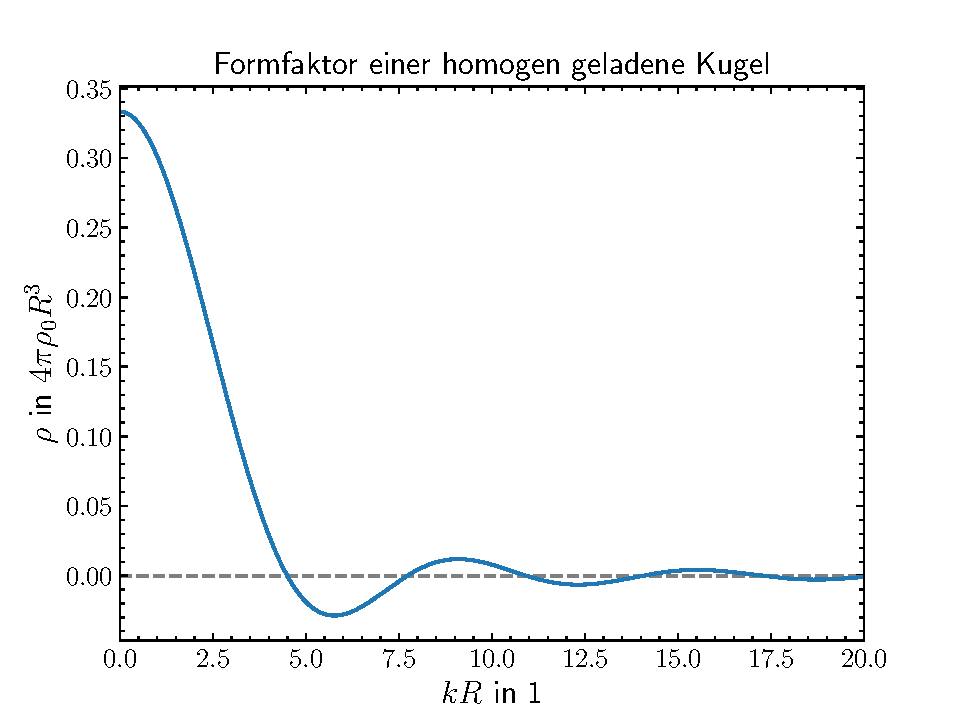
\includegraphics[width=1.0\textwidth]{formfaktor.pdf}
    \caption{Plot}
\end{figure}

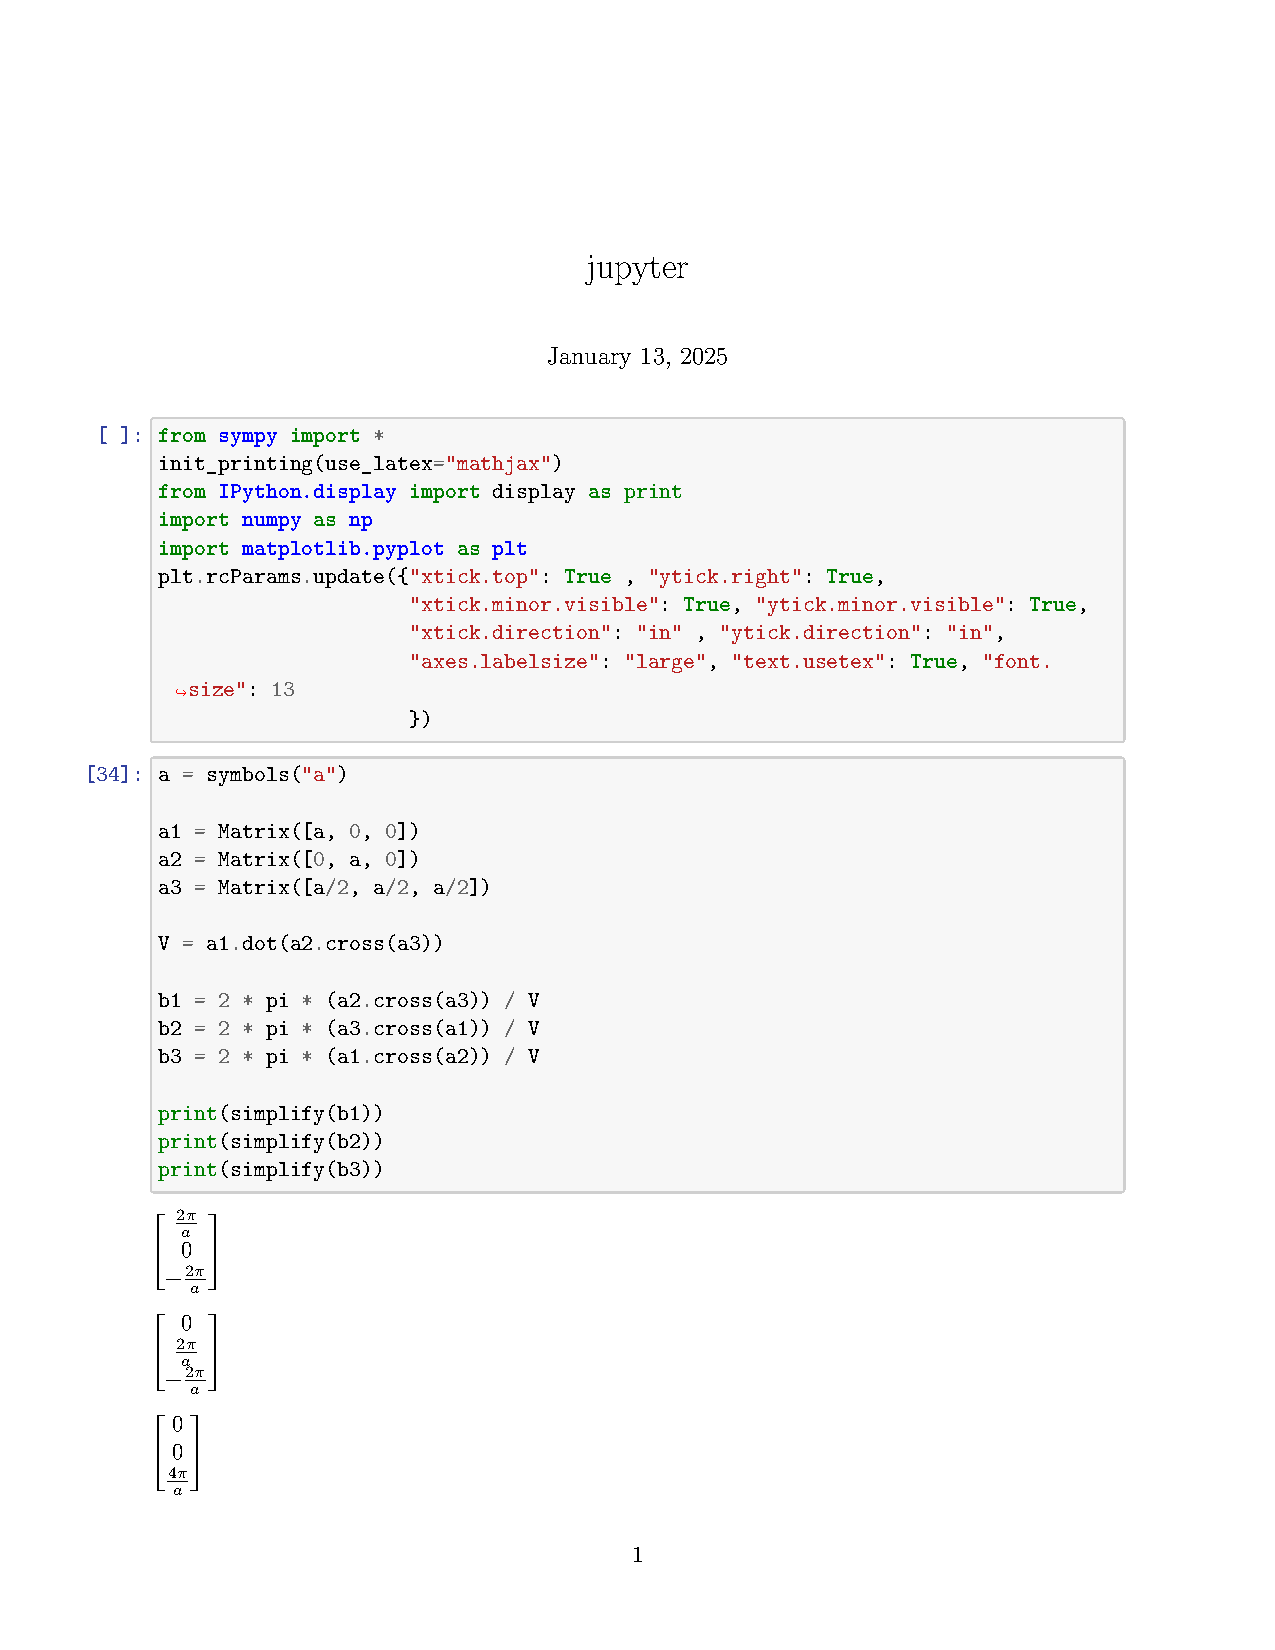
\includepdf[pages=-]{jupyter.pdf}


\end{document}